
\documentclass[ucs]{beamer}

\usetheme{GSyC}
%\usebackgroundtemplate{\includegraphics[width=\paperwidth]{gsyc-bg.png}}


\usepackage[spanish]{babel}  
\usepackage[utf8x]{inputenc}
\usepackage{graphicx}
\usepackage{amssymb} % Simbolos matematicos


% Metadatos del PDF, por defecto en blanco, pdftitle no parece funcionar
   \hypersetup{%
     pdftitle={json},%
     %pdfsubject={Diseño y Administración de Sistemas y Redes},%
     pdfauthor={GSyC},%
     pdfkeywords={},%
   }
%


% Para colocar un logo en la esquina inferior de todas las transpas
%   \pgfdeclareimage[height=0.5cm]{gsyc-logo}{gsyc}
%   \logo{\pgfuseimage{gsyc-logo}}


% Para colocar antes de cada sección una página de recuerdo de índice
%\AtBeginSection[]{
%  \begin{frame}<beamer>{Contenidos}
%    \tableofcontents[currentframetitle]
%  \end{frame}
%}



\begin{document}

% Entre corchetes como argumento opcional un título o autor abreviado
% para los pies de transpa
\title[JSON]{JSON en JavaScript }
%\subtitle{Diseño y Administración de Sistemas y Redes}
\author[GSyC]{Escuela Técnica Superior de Ingeniería de Telecomunicación\\
Universidad Rey Juan Carlos}
\institute{gsyc-profes (arroba) gsyc.urjc.es}
\date[2017]{Noviembre de 2017}


%% TÍTULO
\begin{frame}
  \titlepage
  % Oportunidad para poner otro logo si se usó la opción nologo
  % \includegraphics[width=2cm]{logoesp}  
\end{frame}



%% LICENCIA DE REDISTRIBUCIÓN DE LAS TRANSPAS
%% Nota: la opción b al frame le dice que justifique el texto
%% abajo (por defecto c: centrado)
\begin{frame}[b]
\begin{flushright}
{\tiny
\copyright \insertshortdate~\insertshortauthor \\
  Algunos derechos reservados. \\
  Este trabajo se distribuye bajo la licencia \\
  Creative Commons Attribution Share-Alike 4.0\\
}
\end{flushright}  
\end{frame}



%% ÍNDICE
%\begin{frame}
%  \frametitle{Contenidos}
%  \tableofcontents
%\end{frame}



%the practice of system and network administration
%t limoncelli

%principles of network and system administration
%m burgess


\section{JSON}


%%---------------------------------------------------------------
\begin{frame}[fragile]
\frametitle{JSON}
Es un formato ligero para intercambiar datos, independiente del lenguaje de 
programación y de la plataforma
\begin{itemize}
\item
Estándar abierto, RFC 4627, año 2006
\item
Originalmente se consideraba subconjunto del lenguaje JavaScript y se
denominaba  \emph{JavaScript Object Notation}, aunque ya no es parte de JavaScript
\item
Diseñado como alternativa a XML, más ligero. Actualmente es más popular que XML
\item
Carece de algunas características de XML, por ejemplo gramáticas o diferencia entre texto y metadato 
\end{itemize}

\end{frame}

%%---------------------------------------------------------------
\begin{frame}[fragile]
\frametitle{Value}
\begin{center}
  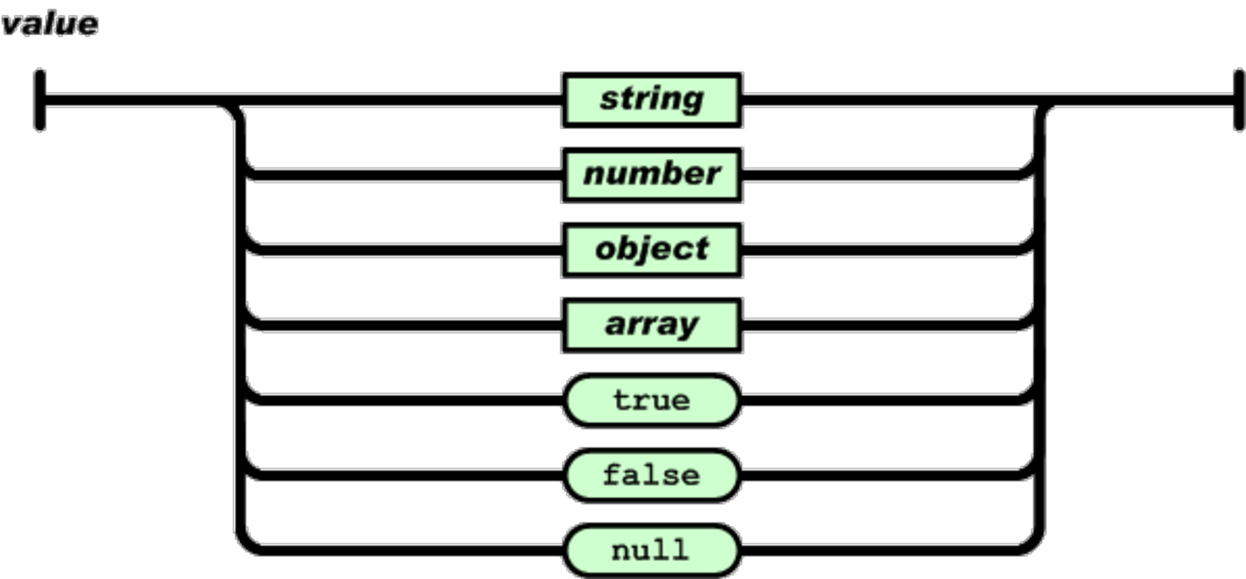
\includegraphics[width=09.0cm]{figs/value}
\end{center}
\begin{flushright}
\begin{tiny}
Fuente:json.org
\end{tiny}
\end{flushright}
\begin{itemize}
\item 
Un valor JSON puede ser un número, una cadena, un array o
un objeto, además de las constantes 
\emph{true},
\emph{false} y 
\emph{null}
\item 
Igual que JavaScript. Excepto que 
\emph{undefined} no es un valor JSON
\end{itemize}
\end{frame}



%%---------------------------------------------------------------

\begin{frame}[fragile]
\frametitle{Number}
\begin{center}
  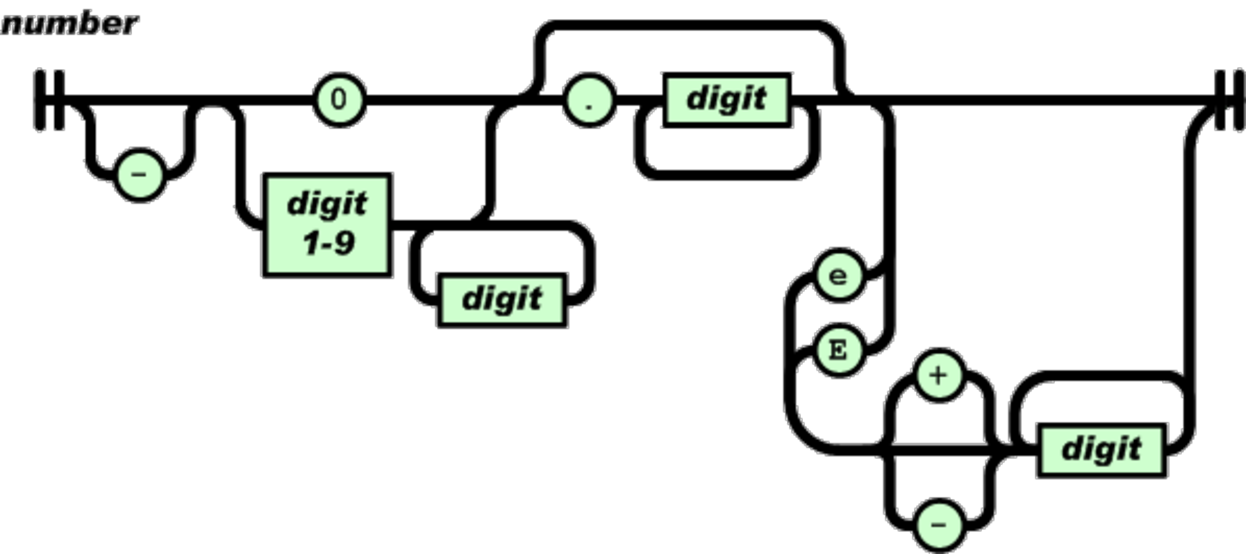
\includegraphics[width=08.5cm]{figs/number}
\end{center}
\begin{flushright}
\begin{tiny}
Fuente:json.org
\end{tiny}
\end{flushright}
\begin{itemize}
\item 
Los números son como las constantes numéricas
de cualquier lenguaje de programación moderno
\end{itemize}
\end{frame}

%%---------------------------------------------------------------

\begin{frame}[fragile]
\frametitle{String}
\begin{center}
  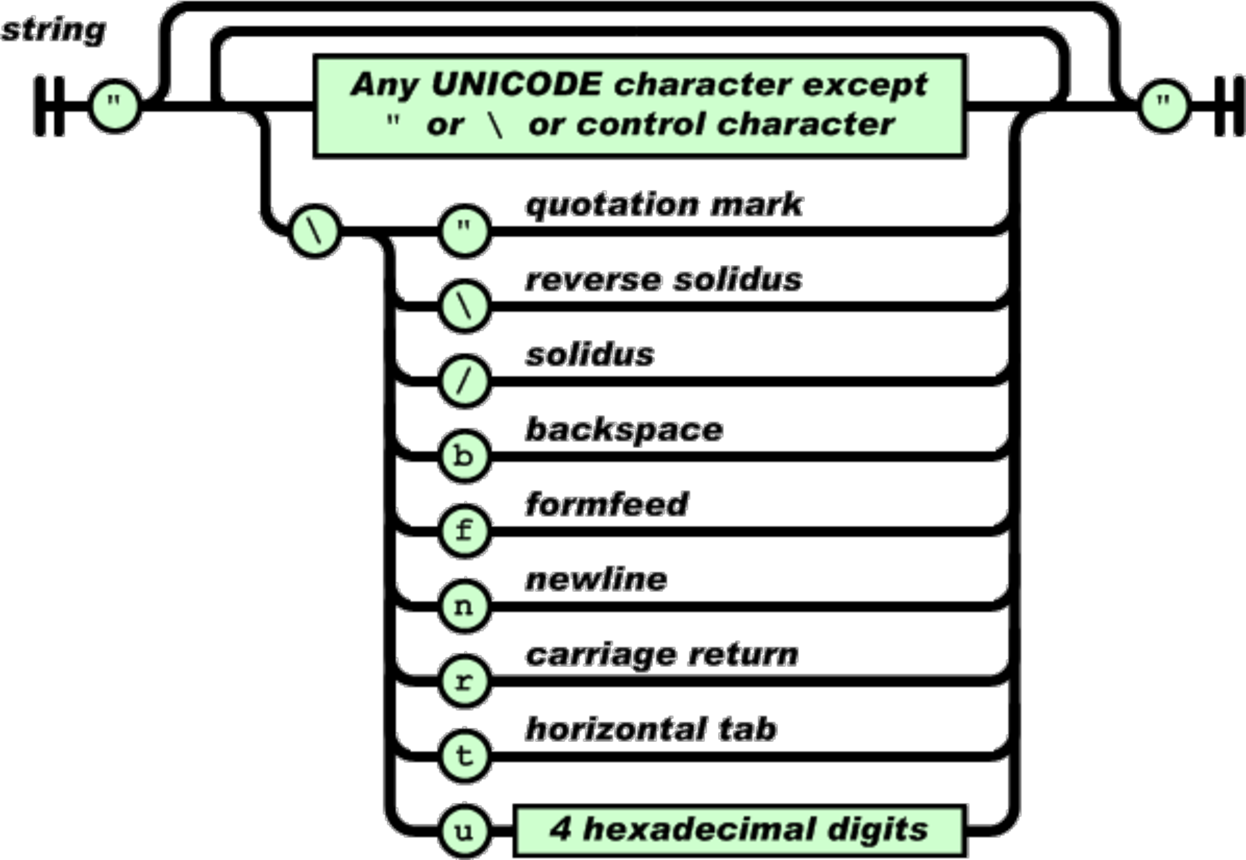
\includegraphics[width=06.3cm]{figs/string}
\end{center}
\begin{flushright}
\begin{tiny}
Fuente:json.org
\end{tiny}
\end{flushright}
\begin{itemize}
\item 
Las cadenas son como las de cualquier lenguaje de programación moderno
\item
El delimitador es la comilla doble

    \begin{itemize}
    \item
JavaScript admite la comilla doble y la simple, aunque la más habitual es la simple
    \end{itemize}
\end{itemize}
\end{frame}

%%---------------------------------------------------------------
\begin{frame}[fragile]
\frametitle{Array}
\begin{center}
  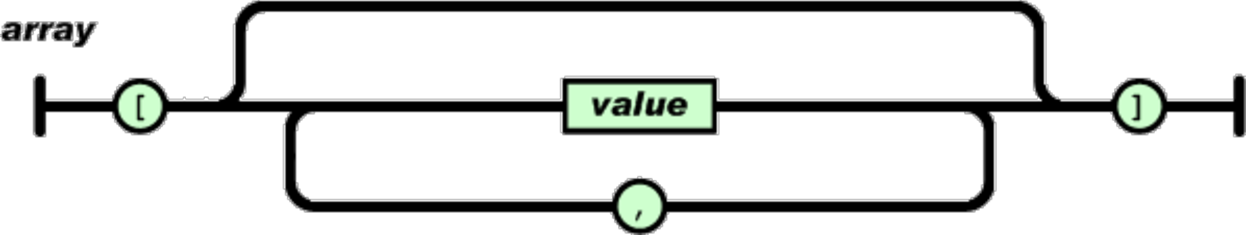
\includegraphics[width=10.5cm]{figs/array}
\end{center}
\begin{flushright}
\begin{tiny}
Fuente:json.org
\end{tiny}
\end{flushright}
\begin{itemize}
\item 
Un array es una secuencia de valores entre corchetes, separados por comas

\item 
Igual que JavaScript
 
\end{itemize}
\end{frame}

%%---------------------------------------------------------------
\begin{frame}[fragile]
\frametitle{Objetos}
\begin{center}
  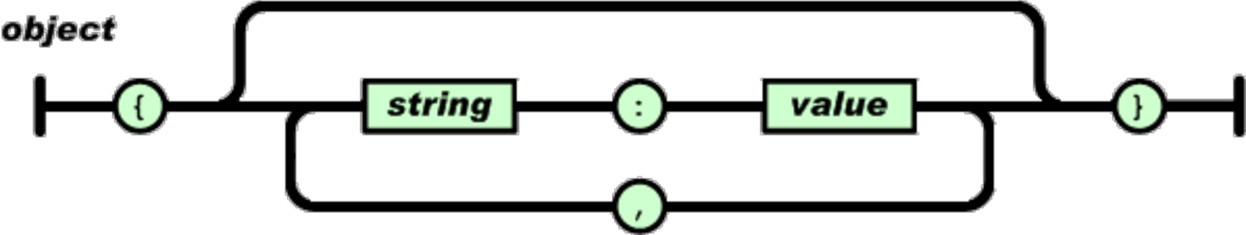
\includegraphics[width=10.5cm]{figs/object}
\end{center}
\begin{flushright}
\begin{tiny}
Fuente:json.org
\end{tiny}
\end{flushright}
\begin{itemize}
\item 
Un objeto es una secuencia de pares clave:valor, separados por comas
\item
Las claves son cadenas
\item
Igual que JavaScript
 
\end{itemize}
\end{frame}


%%---------------------------------------------------------------
\begin{frame}[fragile]
\frametitle{Ejemplos correctos}
\begin{itemize}
\item
  \begin{footnotesize}
  \begin{verbatim}
"hola, mundo"
  \end{verbatim}
  \end{footnotesize}

\item

  \begin{footnotesize}
  \begin{verbatim}
4243.12
  \end{verbatim}
  \end{footnotesize}

\item
  \begin{footnotesize}
  \begin{verbatim}
-947e-5
  \end{verbatim}
  \end{footnotesize}

\item
  \begin{footnotesize}
  \begin{verbatim}
null
  \end{verbatim}
  \end{footnotesize}


\item
  \begin{footnotesize}
  \begin{verbatim}
[1,2,3,4]
  \end{verbatim}
  \end{footnotesize}


\end{itemize}
\end{frame}
%%----------------------------------------------
\begin{frame}[fragile]
\frametitle{}
\begin{itemize}

\item

  \begin{footnotesize}
  \begin{verbatim}
[1, "azul", [1,2,3]]
  \end{verbatim}
  \end{footnotesize}



\item
  \begin{footnotesize}
  \begin{verbatim}
[
    1, 
    "azul", 
    [
        1, 
        2, 
        3
    ]
]
  \end{verbatim}
  \end{footnotesize}



\item
  \begin{footnotesize}
  \begin{verbatim}
["as" ,   "dos", "tres"]
  \end{verbatim}
  \end{footnotesize}


\item
  \begin{footnotesize}
  \begin{verbatim}
["sota", "caballo", "rey"]
  \end{verbatim}
  \end{footnotesize}

\item
  \begin{footnotesize}
  \begin{verbatim}
[
    "sota",
    "caballo",
    "rey"
]
  \end{verbatim}
  \end{footnotesize}

\end{itemize}

\end{frame}



%%---------------------------------------------------------------
\begin{frame}[fragile]
\frametitle{}
\begin{itemize}




\item
  \begin{footnotesize}
  \begin{verbatim}
{ "nombre":"Juan", "apellido":"Pérez"}
  \end{verbatim}
  \end{footnotesize}
\item
  \begin{footnotesize}
  \begin{verbatim}
{ "v1":true, "v2":null, "v3":false}
  \end{verbatim}
  \end{footnotesize}
\item
  \begin{footnotesize}
  \begin{verbatim}
{ "nombre": "Juan", "notas":[5.5, 7.2, 6.1]}
  \end{verbatim}
  \end{footnotesize}
\item
  \begin{footnotesize}
  \begin{verbatim}
{
    "nombre": "Juan", 
    "notas": [
        5.5, 
        7.2, 
        6.1
    ]
}
  \end{verbatim}
  \end{footnotesize}
\end{itemize}

\end{frame}


%%---------------------------------------------------------------
\begin{frame}[fragile]
\frametitle{Ejemplos incorrectos}
\begin{itemize}
\item
  \begin{footnotesize}
  \begin{verbatim}
True
  \end{verbatim}
  \end{footnotesize}
\item

  \begin{footnotesize}
  \begin{verbatim}
'hola, mundo'
  \end{verbatim}
  \end{footnotesize}

\item
  \begin{footnotesize}
  \begin{verbatim}
{"hola,mundo"}
  \end{verbatim}
  \end{footnotesize}

\item
  \begin{footnotesize}
  \begin{verbatim}
{1:"uno", 2:"dos"}
  \end{verbatim}
  \end{footnotesize}
\end{itemize}
\end{frame}




\section{JSONP}

%%---------------------------------------------------------------
\begin{frame}[fragile]
\frametitle{Same-origin policy}

\emph{Same-origin policy}
es una norma que aparece en Netscape 2 (año 1995), que se ha convertido en un estándar.
Consiste en que el código JavaScript solo puede acceder a datos que provengan del mismo
origen desde el que se ha cargado el script


    \begin{itemize}
    \item
Se entiende por \emph{origen} el mismo protocolo, máquina y puerto
    \end{itemize}


Ejemplo

    \begin{itemize}
    \item
El usuario accede a una página web en
\emph{molamazo.com},

    \item
Esta página web puede tener código JavaScript que acceda a datos que estén en
\emph{molamazo.com},
pero
solamente en este sitio

    \item
No puede acceder a datos en
\emph{bancofuenla.es}


    \begin{itemize}
    \item
De lo contrario, una vez que el usuario se autentica en
\emph{bancofuenla}
con una página de
\emph{bancofuenla},
un script malicioso en
\emph{molamazo}
podría acceder a información sensible en
\emph{bancofuenla}
    \end{itemize}
    \end{itemize}


\end{frame}




%%---------------------------------------------------------------
\begin{frame}[fragile]
\frametitle{JSOP}

JSONP (\emph{JSON with padding, JSON con relleno})  es una técnica que permite que una página web obtenga datos desde un
sitio web distinto al suyo, sin vulnerar la
\emph{same-origin policy}


    \begin{itemize}
    \item
Es un protocolo del año 2005, soluciona el problema pero no es especialmente elegante. También tiene algunos
problemas de seguridad potenciales

    \item
Una alternativa más avanzada pero menos extendida es CORS,
\emph{Cross-origin resource sharing}
    \end{itemize}



JSONP
requiere de la colaboración del servidor. Es necesario que un servidor ofrezca datos no solo
en JSON, también en JSONP

\end{frame}


%%---------------------------------------------------------------
\begin{frame}[fragile]
\frametitle{}
JSONP
se basa en que la
\emph{same-origin policy}
se aplica solo a datos, no a scripts

\begin{itemize}
    \item
Ejemplo:
un script descargado desde
\emph{molamazo.com},
no puede
descargar datos
desde
\emph{bancofuenla.es},
pero sí puede descargar otro script

    \item
Se entiende que esto no es especialmente peligroso.
\emph{Bancofuenla}
podría enviar una contraseña a una página web, como un dato,  esperando que la lea el usuario.

Pero en un script nunca debería haber información sensible

    \end{itemize}

\end{frame}

%%----------------------------------------------
\begin{frame}[fragile]


Ejemplo de uso de JSOP

\begin{itemize}
    \item
Enviar \verb|3| no está permitido, es un dato.

    \item
Pero la cadena \verb|"f(3)"| no es un dato. Es un script.
Se puede enviar.


    \begin{itemize}
    \item
Si
\emph{bancofuenla}
accede a enviar
\verb|"f(3)"|
como dato JSON, sabe que esta información podría ser usada por un script de
cualquier otro sitio, p.e.
\emph{molamazo}. Por tanto, nunca enviará de este modo información sensible

    \item
Un problema disintinto, que JSONP no contempla, es que sea
\emph{bancofuenla}
quien aproveche esto para enviar código dañino
    \end{itemize}
    \end{itemize}


\end{frame}

%%----------------------------------------------
\begin{frame}[fragile]


En JSONP, el cliente solicita un dato a un sitio web
( en nuestro ejemplo, \emph{bancofuenla}), y también
le indica el nombre de la función en la que se \emph{envuelve} el dato.

\begin{itemize}
    \item
Esto se hace con un parámetro que suele denominarse  \verb|callback|

Una petición podría ser


  \begin{scriptsize}
  \begin{verbatim}
bancofuenla.es/divisas.html?par=USDEUR&fecha=hoy&callback=procesaDivisas
  \end{verbatim}
  \end{scriptsize}

    \item
A la que el servidor podría responder

\verb|procesaDivisas(0.865)|

    \item
\verb|procesaDivisas()|
será una función en el script cliente, que tratará el dato (0.865)

\end{itemize}

\end{frame}





\section{Funciones para procesar JSON}
%%---------------------------------------------------------------
\begin{frame}[fragile]
\frametitle{Conversión de objeto en cadena JSON}
En JavaScript,
para convertir un objeto en una cadena JSON
usamos la \emph{built-in function} JSON.stringify

  \begin{scriptsize}
  \begin{verbatim}
'use strict'
let lista=[ "sota", "caballo", "rey" ];
console.log(typeof(lista),lista);
// object ["sota","caballo","rey"]

let cadena=JSON.stringify(lista);
console.log(typeof(cadena),cadena);
// string ["sota","caballo","rey"]
  \end{verbatim}
  \end{scriptsize}

\end{frame}


%%---------------------------------------------------------------
\begin{frame}[fragile]
\frametitle{Conversión de cadena JSON en objeto}
Para convertir una cadena de texto con un JSON en un objeto
JavaScript, disponemos de la 
\emph{built-in function} JSON.parse

  \begin{scriptsize}
  \begin{verbatim}
'use strict'
let cadena='{ "nombre":"redes", "curso":1, "horario":["L1500", "X1700"] }'
console.log(typeof(cadena),cadena);
 // string { "nombre":"redes", "curso":1, "horario":["L1500", "X1700"] }

let objeto=JSON.parse(cadena);
console.log(typeof(objeto),objeto);
/*
object { nombre: 'redes',
  curso: 1,
  horario: [ 'L1500', 'X1700' ] }
*/

  \end{verbatim}
  \end{scriptsize}

Si la cadena no cumple el formato JSON, se genera una excepción
\emph{SyntaxError}

\end{frame}
\end{document}

